\documentclass{article}
\usepackage{amsfonts}
\usepackage{graphicx}
\usepackage[margin=1in]{geometry}
\usepackage{bm}
\usepackage{amsmath}

\author{Quang P. Nguyen}
\title{Supplementary Materials}
\begin{document}
\maketitle

\section{Distribution of cILR}
\begin{figure}[h]
    \centering
    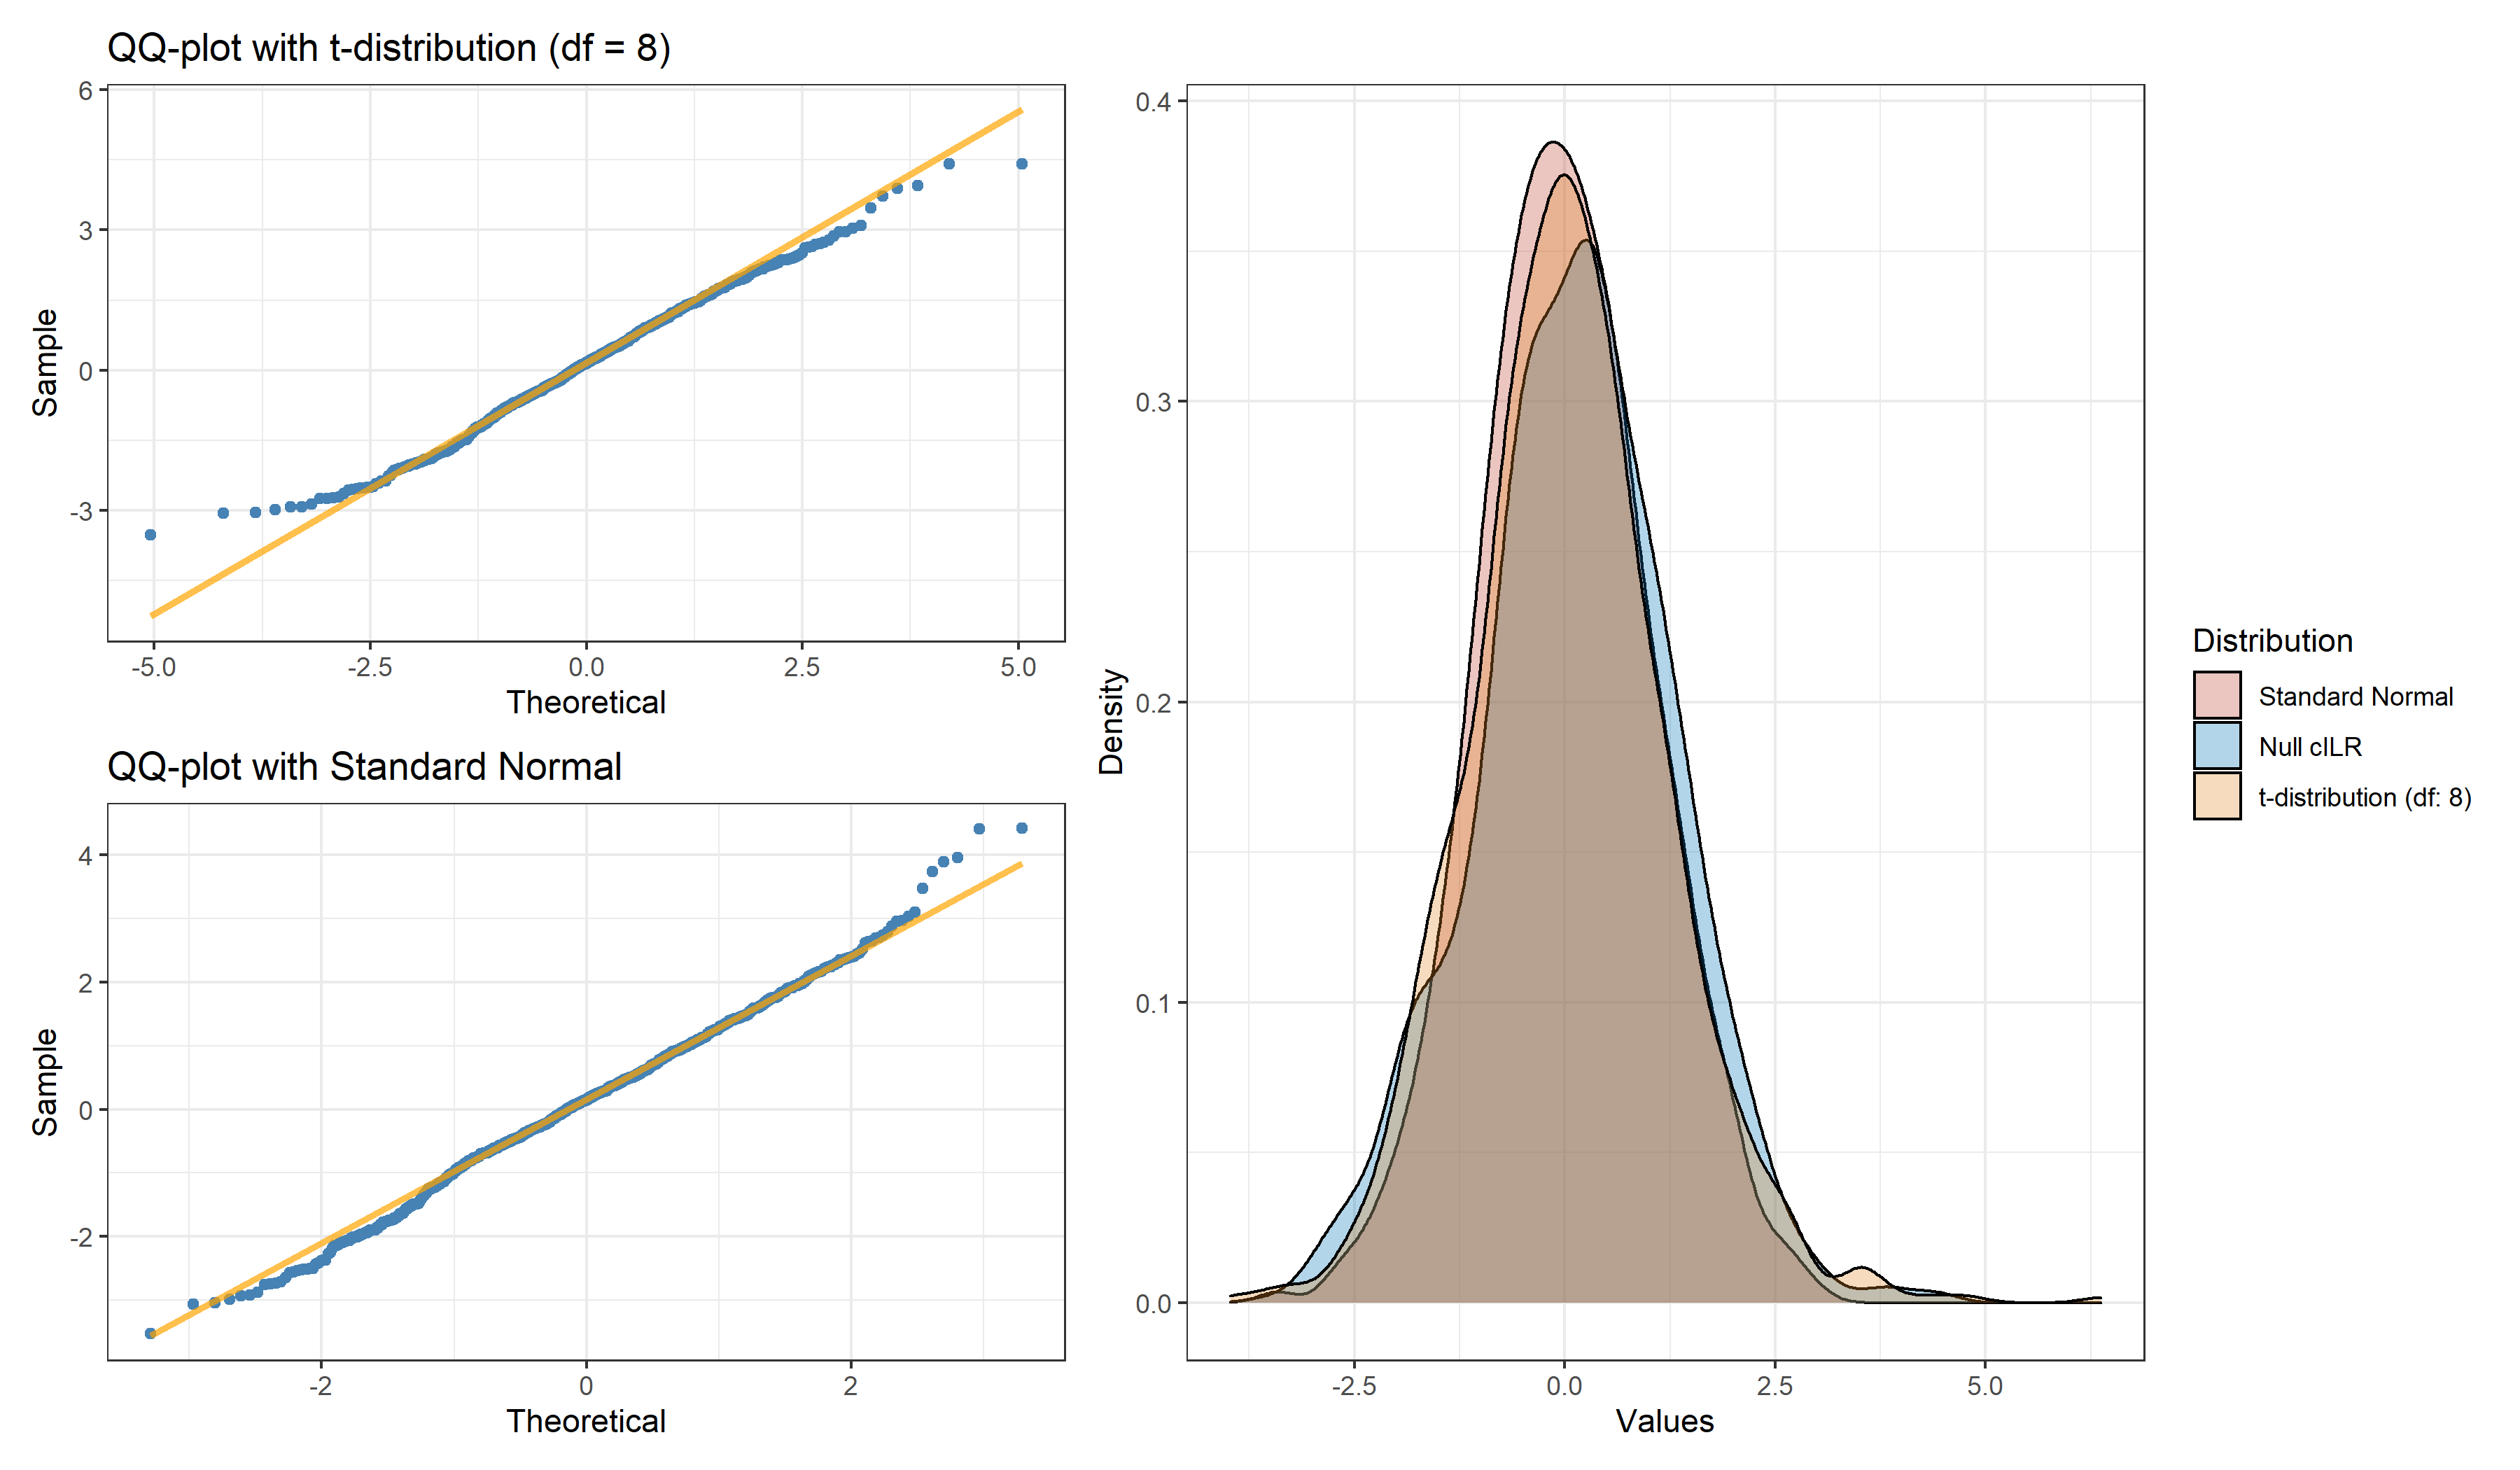
\includegraphics[width=0.8\linewidth]{figures/null_distribution.png}
    \caption{The distribution of cILR statistic under the null. We compared the null distribution of the test statistic and compare it with the standard normal distribution, and the t-distribution with degrees of freedom fitted to cILR scores using the maximum likelihood method}
\end{figure}

\section{Simulation Design}
We simulated microbiome relative abundance data using the NorTA similar to \cite{cario}. Using this method, we can generate synthetic microbial counts that incorporates a complex correlation structure and multiple types of marginals. Specifically, we chose our marginals to be the zero-inflated negative binomial distribution based on results by Kurtz et al. \cite{kurtz2015}

\noindent We fit the the parameters to our marginal model based on 16S rRNA sequencing of the V3-V5 region from stool samples in the Human Microbiome Project (HMP). This data was accquired via the \emph{HMP16S} package in R \cite{schiffer2019}. 

\begin{figure}[h]
    \centering
    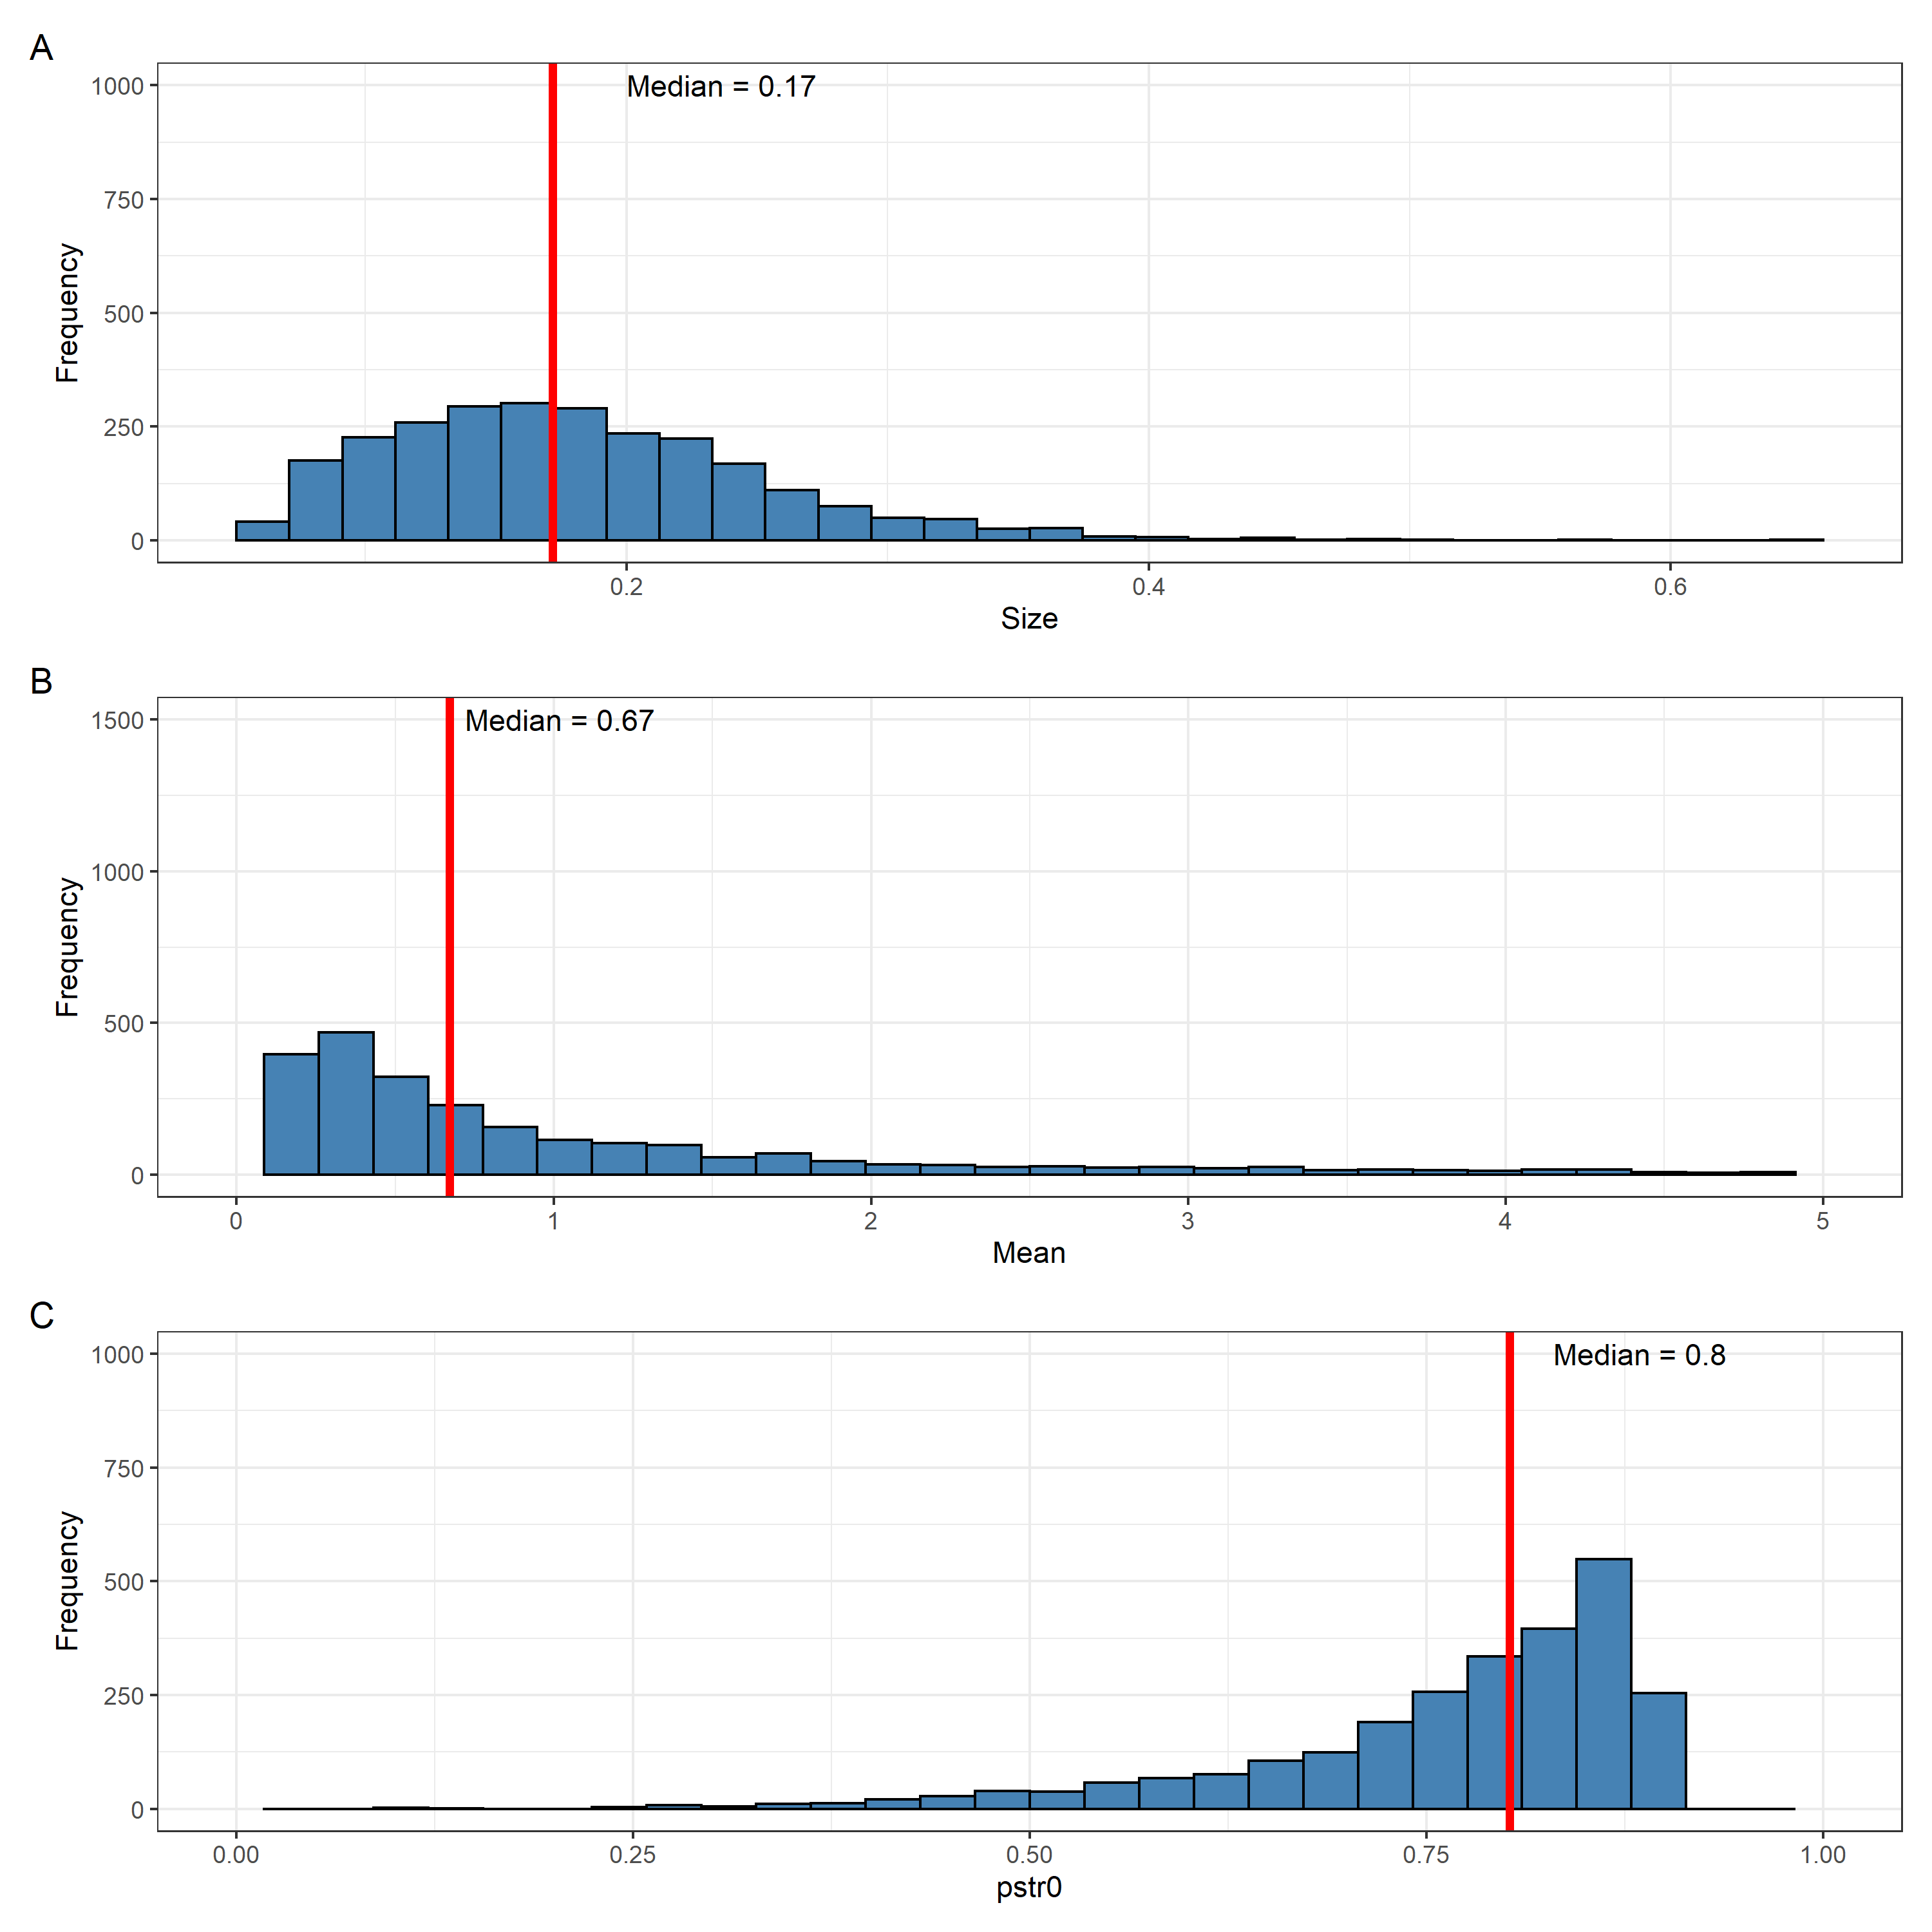
\includegraphics[width=0.6\linewidth]{figures/HMP_fit.png}
    \caption{Distribution of each parameter of the zero inflated negative binomial distribution fitted to HMP16S data. The parameters are size (panel A), mean (panel B) and probability of 0 (panel C)}
\end{figure}


\newpage
\bibliography{tax_agg}{}
\bibliographystyle{plain}

\end{document}